\chapter{Qualitätsmerkmale von Software}
\label{cha:qualitaetsmerkmale}

%----------------------------------
%
% Definition von Qualität
%
%----------------------------------
    \section{Definition von Qualität}
    \label{sec:definitionQualitaet}

        Der Begriff Qualität wird im Alltag häufig und in verschiedenen Situationen verwendet. Daher soll hier eine Grunddefinition des Qualitätsbegriffs gegeben werden, der im Rahmen der vorliegenden Arbeit verwendet wird.

        Es kann gesagt werden, dass Qualität
            \begin{itemize}
                \item \enquote{eine Menge von Eigenschaften repräsentiert, die einem Produkt oder Verfahren immanent oder beigegeben ist.
                \item einer der Maßstäbe ist, mit dem der Kunde seine Kaufentscheidung herbeiführt.
                \item ein Faktor ist, der in intensiver Wechselwirkung mit der Wettbewerbssituation und Leistungsfähigkeit eines Anbieters steht.}\footnotemark
            \end{itemize}

            \footnotetext{Pfeifer (Qualitätssicherung).}

        Dies verfeinert die Definition der \emph{International Organisation for Standardization} (ISO) 9000: \enquote{Qualität ist der Grad, in dem ein Satz inhärenter Merkmale Forderungen erfüllt.}\footnote{Glinz (Software Engineering), S.115.} Für Qualität bedeutet das, dass einem Werksstück, Prozess oder auch einer Software messbare und nicht messbare Eigenschaften inne wohnen. Bei Software unterscheidet man beispielsweise zwischen messbaren, funktionalen Anforderungen und nicht messbaren, nicht funktionalen Anforderungen. Ein Beispiel für eine funktionale Anforderung ist die Antwortzeit eines Programms, während ein gutes User Interface einer nicht funktionalen Anforderung entspricht. Inhärent sind Merkmale, die sich nach Auslieferung nur sehr schwer oder gar nicht verändern lassen, während der Preis als Beispiel für ein nicht-inhärentes Merkmal sehr frei zu gestalten ist.

        Ein wichtiges Merkmal der vorausgegangenen Definition ist allerdings die Qualität als Merkmal der Kundenbeeinflussung. Dabei stellt sie sich als Merkmal dar, dass für oder auch gegen die Kaufentscheidung eines bestimmten Produktes spricht. Als Softwarehersteller ist somit eine Sicherung der Qualität unumgänglich, um nachhaltig am Markt zu agieren.

        So wird Qualität im Rahmen dieser Arbeit als eine Eigenschaft des fertigen Produkts, in diesem Fall der Software, angesehen, die nachträglich nur durch sehr viel Aufwand verändert werden kann. Qualität ist ein Maßstab auf dessen Grundlage Kunden eine Kaufentscheidung treffen, abhängig davon, ob die eigenen Anforderungen an das Produkt erfüllt sind.

%----------------------------------
%
% Vorstellung der Qualitätsmerkmale
%
%----------------------------------
    \section{Vorstellung der Qualitätsmerkmale}
    \label{sec:vorstellungMerkmale}

        Die Produktqualität ist, wie zuvor gezeigt, ein wichtiges Merkmal zum Bilden und Fortbestehen eines Unternehmens. Im Folgenden soll die Qualität einer Software messbar gemacht werden.

        Die ISO 9126 stellt hierzu sechs Charakteristiken bereit, auf deren Grundlage die Qualität von Software bewertet werden kann. Die Charakteristiken sind zusätzlich in insgesamt 27 Unterdimensionen untergliedert. Es werden nun alle Obercharakteristiken betrachtet und im Anschluss drei Merkmale ausgewählt, die im Rahmen dieser Arbeit betrachtet werden. Die Definitionen der Unterdimensionen befinden sich im Glossar.

        \subsection{Funktionalität}

            \begin{quote}
              \enquote{The capability of the software product to provide functions which meet stated and implied needs when the software is used under specified conditions.}\footnote{ISO 9126-1 (Information technology), S.7.}
            \end{quote}

            Die Charakteristik \emph{Funktionalität} gibt den Einsatzzweck der Software an. Beispielsweise ist eine Funktionalität einer Buchhaltungssoftware die Berechnung einer Gewinn- und Verlustrechnung. Im Gegensatz zu den folgenden Charakteristiken gibt diese an, was die Software tut, anstatt zu sagen, auf welche Weise sie etwas tut.

            Darunter fallen die Abdeckung der gestellten Anforderungen an Funktionalität und Genauigkeit, sowie Sicherheitsaspekte.\footnote{Vgl. ISO 9126-1 (Information technology), S.8.} Im Falle der SAP SE hat ein Softwareprodukt beispielsweise die Funktion der Geschäftspartnerverwaltung und sollte somit alle fachlich an sie gestellten Anforderungen bedienen. Außerdem sollte bei einer identischen Eingabe stets ein identisches, erwartetes Resultat entstehen. Durch den Scope (engl. für Umfang), der zu Beginn eines Projektes erstellt wird, ist diese Charakteristik meist schon zu Beginn eines Projekts genau spezifiziert.

        \subsection{Verlässlichkeit}

            \begin{quote}
              \enquote{The capability of the software product to maintain a specified level of performance when used under specified conditions.}\footnote{ISO 9126-1 (Information technology), S.8.}
            \end{quote}

            Die Charakteristik \emph{Verlässlichkeit} gibt die Fähigkeit einer Software an, unter den festgelegten Umweltbedingungen immer in einem vorher festgelegten Rahmen zu reagieren. In mittlerweile veraltetenen Definitionen der ISO Normen bezieht sich die Verlässlichkeit darauf, eine bestimmte, benötigte Funktion auszuführen.

            Das Ziel der Entwickler ist eine Software, die jederzeit in dem erwarteten Umfang reagiert und falsche Eingaben, falsche Benutzungsanweisungen und ungültige Datensätze verkraftet oder verhindert. Software ist genau dann verlässlich, wenn keine Fehler durch Defekte in dieser auftreten, keine Angriffe, bewusst oder unbewusst, von außen oder innen möglich sind und sämtliche Daten auch nach einem Systemabsturz wieder herstellbar sind.\footnote{Vgl. ISO 9126-1 (Information technology), S.9.}

            Unternehmen der Finanzindustrie stellen hohe Anforderungen an die Verlässlichkeit ihrer IT Systeme. Ebenso ist die zuverlässige Ausführung von Prozessen bei der Verarbeitung von Zahlungsströmen u.ä. unverzichtbar.
            Derzeit werden Softwarelandschaften eingesetzt, die in den 1970er Jahren aufgebaut wurden und seitdem im Stand gehalten und erweitert werden.\footnote{Vgl. TOGAF/Bian (Integrating TOGAF with BIAN), S.10.} Die auf Mainframes\footnote{Siehe Glossar.} aufgebauten Architekturen sind sehr teuer in der Wartung und Instandhaltung, aber gewährleisten eine hohe Verfügbarkeit von bis zu 99.999\%.\footnote{Vgl. Symonds (Mainframes), S.12.}
            %Dies bedeutet, dass ein Mainframe nur circa 5,26 Minuten pro Jahr nicht zu erreichen ist. IBM gibt für ihre Mainframes zudem eine durchschnittliche Zeit zwischen Fehlern von 20 bis 30 Jahren an. Außerdem werden Operationen häufig mehrfach gleichzeitig durchgeführt und die Ergebnisse verglichen. Somit sind fehlerhafte Berechnungen nahezu ausgeschlossen.

        \subsection{Benutzerfreundlichkeit}

            \begin{quote}
              \enquote{The capability of the software product to be understood, learned, used and attractive to the user, when used under specified conditions.}\footnote{ISO 9126-1 (Information technology), S.9.}
            \end{quote}

            \emph{Benutzerfreundlichkeit} sagt aus, dass ein fachlich versierter Anwender intuitiv die Funktion des Programms erkennt und es verwenden kann. Dabei soll der Anwender nach Möglichkeit ein gutes Gefühl haben und die Software als schön bezeichnen.

            Aus dem Privatleben sind geschäftliche Anwender inzwischen einfache, intuitive Oberflächen gewöhnt und tragen diese Anforderung ins Unternehmen.\footnote{Vgl. CITO Research (Business Intelligence), S.1.} Außerdem werden mehr mobile Geräte in Unternehmen verwendet. Um alle Daten, zu jeder Zeit und an jedem Ort zur Verfügung zu haben, werden die Daten häufig in der Cloud\footnote{Siehe Glossar.} bereitgestellt und über webbasierte Applikationen angezeigt.

            Die SAP SE verfolgt die Strategie, dass sich die Oberflächen zwischen mobilen Geräten und Computern nicht unterscheiden und keine Daten auf dem Gerät liegen. Durch einheitliche Oberflächen soll die Produktivität der Nutzer erhöht werden und die Einarbeitungszeit reduziert werden.
            Das Ziel der SAP SE ist es, durch eine intuitive Menüführung beim Endbenutzer einen Produktivitätszuwachs zu erreichen, dadurch, dass dieser schnell und sicher durch die Oberfläche navigieren kann. Durch leicht verständliche Oberflächen soll zudem die zur Einarbeitung benötigte Zeit reduziert werden. Somit wird im Idealfall der Schulungsbedarf des Kunden reduziert.\footnote{Vgl. Deck (User Interface Technologies), S.14ff.}

        \subsection{Effizienz}

            \begin{quote}
              \enquote{The capability of the software product to provide appropriate performance, relative to the amount of resources used, under stated conditions.}\footnote{ISO 9126-1 (Information technology), S.10.}
            \end{quote}

            Der Faktor \emph{Effizienz} drückt das Verhältnis zwischen der Performanz der Software und den dafür verbrauchten Ressourcen aus.\footnote{Vgl. ISO 9126-1 (Information technology), S.10.} Die Effizienz steigt, wenn die Performance bei gleichbleibendem Ressourcenverbrauch steigt, oder, wenn bei gleichbleibender Performance der Ressourcenverbrauch sinkt und umgekehrt.

            Um selbst bei umfangreichen Datenabfragen und Berechnungen eine geringe Antwortzeit zu gewährleisten verfolgt die SAP SE den Trend der In-Memory Datenhaltung. Die SAP SE verwendet hierzu die Datenbanktechnologie \emph{High-Performance Analytical Appliance} (HANA)\footnote{Siehe Glossar.}. Trotz der gestiegenen Ressourcennutzung ist der Performance Gewinn größer, um deren Verwendung zu rechtfertigen. Gerade im Umgang mit Massendaten, die im Finanzbereich anfallen ist eine effiziente Datenhaltung und Verarbeitung sehr wichtig.\footnote{Vgl. SAP SE (HANA in Banking), S.5.}

        \subsection{Wartbarkeit}

            \begin{quote}
              \enquote{The capability of the software product to be modified. Modifications may include corrections, improvements or adaptation of the software to changes in environment, and in requirements and functional specification.}\footnote{ISO 9126-1 (Information technology), S.10.}
            \end{quote}

            Die \emph{Wartbarkeit} einer Software wird anhand der Möglichkeit bewertet, Korrekturen, Verbesserungen und neue Funktionen einzuspielen. Außerdem sollte die Software an neue Anforderungen, wie neue Prozesse oder neue umliegende Systeme anpassbar sein.\footnote{Vgl. ISO 9126-1 (Information technology), S.10.}

            Die SAP SE bietet ihre Software mit Wartungsverträgen an, die die Aktualität der Software über mehrere Jahre garantiert. Ein Beispiel für eine Erweiterung ist die Umstellung der innereuropäischen Banküberweisungen auf SEPA\footnote{Single Euro Payments Area.}. Hier mussten unter anderem die bisher 10-stelligen numerischen Kontonummern auf eine 22-stellige alphanumerische Zeichenkette umgestellt werden.\footnote{Vgl. Ruth (SEPA).}

        \subsection{Portierbarkeit}

            \begin{quote}
              \enquote{The capability of the software product to be transferred from one environment to another.}\footnote{ISO 9126-1 (Information technology), S.11.}
            \end{quote}

            Die \emph{Portierbarkeit} der Software ist besonders hoch, wenn sie so universell programmiert ist, dass sie ohne oder mit minimalem Aufwand auf verschiedenen Infrastruktur und Software Plattformen verwendet werden kann.\footnote{Vgl. ISO 9126-1 (Information technology), S.11.}

            Für die SAP SE als Anbieter von Standardsoftware ist dies einer der Hauptfaktoren zur Entwicklung von Software, da dies die Grundlage zur Wiederverwendung von entwickelten Softwarebausteinen bildet.

%----------------------------------
%
% Diskussion und Auswahl von Qualitätsmerkmalen
%
%----------------------------------

    \section{Diskussion und Auswahl von Qualitätsmerkmalen}
    \label{sec:diskussionMerkmale}

        Im Folgenden werden die in \autoref{sec:vorstellungMerkmale} vorgestellten Qualitätsmerkmale bewertet und deren jeweilige Relevanz für das in dieser Arbeit betrachtete Projekt evaluiert. Hierzu werden drei Merkmale herausgestellt, die im weiteren Verlauf dieser Arbeit zur Bewertung der Software verwendet werden. \autoref{abb:merkmale} zeigt alle Merkmale zur Bewertung von Qualität. Die Merkmale, die in dieser Arbeit weiter betrachtet werden, sind in Gold hervorgehoben.

        \begin{figure}[!htbp]
                \begin{center}
                    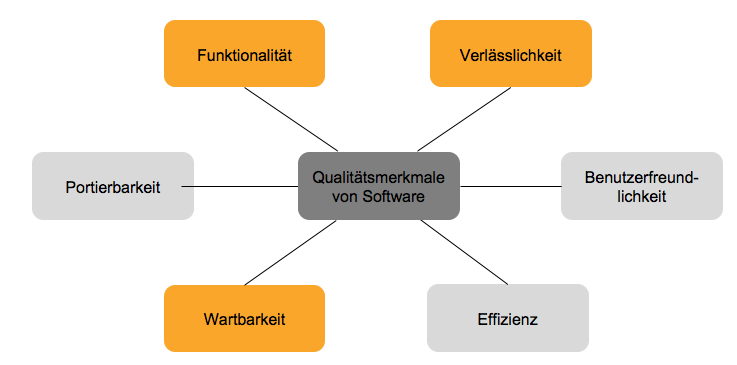
\includegraphics[width=11cm]{Abbildungen/merkmale}
                    \caption[Qualitätsmerkmale von Software]{Qualitätsmerkmale von Software}
                    \label{abb:merkmale}
                \end{center}
        \end{figure}

        \subsection{Funktionalität}

            Funktionalität bewertet den Funktionsumfang der Software. Kunden kaufen Software in der Annahme, dass diese einen Mehrwert für sie darstellt. Das bedeutet, dass die Software die Arbeit des Kunden erleichtert oder die Qualität der Arbeit erhöht. Damit ein Mehrwert geschaffen werden kann, müssen die geforderten Funktionen abgedeckt sein. Eine Software zur Verwaltung von Geschäftspartnern würde keinen Mehrwert liefern, wenn es nicht möglich wäre neue Geschäftspartner anzulegen. Sollte Software für den Kunden jedoch keinen Mehrwert darstellen, gibt es keinen Reiz in diese zu investieren. Eine Software, die die funktionalen Erwartungen des Kunden erfüllt ist somit leichter zu vertreiben.

            Sollte die Software dagegen deutlich mehr Funktionen anbieten als tatsächlich genutzt werden, kann es sein, dass der Anwender von der Funktionalität der Software überfordert ist und die Produktivität somit wieder sinkt. Jede Funktion, die über die Bedürfnisse des Kunden hinausgeht, stellt somit Entwicklungsaufwand dar, der die Kaufbereitschaft des Kunden nicht weiter erhöht, sondern sogar reduzieren kann.

            Für die Entwicklung der Software bedeutet dies, dass die Funktionen, die der Kunde wünscht, implementiert sein sollen, aber keine oder kaum darüber Hinausgehende. Somit wird der Entwicklungsaufwand auf das nötigste reduziert und die Zufriedenheit des Kunden optimiert.
            Um diese Ziele zu erreichen muss die Funktionalität im Rahmen der Softwareentwicklung betrachtet werden und ist somit das erste Bewertungskriterium, dass im weiteren Verlauf dieser Arbeit betrachtet wird.

        \subsection{Verlässlichkeit}

            Durch den bisherigen Einsatz von Mainframes im betrachteten Unternehmen im Bereich der Bausparkasse sind Anwender und Kunden eine hohe Zuverlässigkeit der Software bezüglich der Erreichbarkeit und der Korrektheit der ausgegebenen Ergebnisse gewohnt. Da im Rahmen von Bauspar- und Baufinanzierungsverträgen große Geldbeträge verarbeitet werden, ist es wichtig, dass bei der Verarbeitung eben dieser keine Fehler auftreten. Ein Verlust von Daten, wie Kontoständen oder Personendaten, wäre ebenfalls sehr kritisch, da dies das Vertrauen der Kunden reduziert und diese weniger Produkte nachfragen.

            Die Verfügbarkeit der Software ist im Fall der Bausparkasse jedoch nachrangig, da es sich um langfristig orientierte Geschäfte handelt, die meist keine unmittelbaren Reaktionen erfordern.

            Für die Software ist es im betrachteten Rahmen wichtig, dass keine Fehler produziert werden und keine Daten verloren gehen können, da daraus sehr teure und umständlich zu rekonstruierende Fehler entstehen können. Eine hohe Verlässlichkeit der Software ist damit das zweite betrachtete Bewertungskriterium für die Qualität der Software.

        \subsection{Benutzerfreundlichkeit}

            Benutzerfreundlichkeit wird hauptsächlich durch die Anwendungsoberfläche bestimmt. Die Implementierung von Software ermöglicht es zudem, die Anwendungsoberfläche unabhängig von der Datenhaltung und der Datenverarbeitung zu erstellen. Dies geschieht in einer so genannten 3-Schichten-Architektur\footnote{Siehe Glossar.}. Daher kann die Benutzeroberfläche unabhängig von der zugrunde liegenden Programmlogik implementiert und verändert werden.\footnote{SAP SE (R/3 Architektur).}

            Eine intuitive und einfache Benutzeroberfläche kann die Zufriedenheit und Produktivität der Anwender erhöhen, da diese weniger Fehler machen und somit der Schulungsbedarf geringer ist. Allerdings können die Anwender auch während der Einführungsphase der Software geschult werden, sodass sich hieraus ein Einmalaufwand entwickelt. Eine benutzerfreundliche Oberfläche gibt somit den Anwendern ein besseres Gefühl und verringert Aufwand vorab.

            Die SAP SE setzt bei ihrer Software auf festgelegte Design-Richtlinien, die im Rahmen des Fiori\footnote{Siehe Glossar.} Paradigmas vorgegeben sind. Das Entwicklungsteam der Anwendungslogik hat in diesem Fall nur wenig Einfluss auf die Entwicklung der Benutzeroberfläche. Das Design und die Benutzerfreundlichkeit der Software sind daher bei der Entwicklung der Anwendung nachrangig und werden im Rahmen dieser Arbeit nicht betrachtet.

        \subsection{Effizienz}

            Bauspar- und Baufinanzierungsverträge sind meist langfristig orientiert. Die Kunden informieren sich häufig im Rahmen einer umfassenden Beratung und holen meist Vergleichsangebote ein. Bei den bisher genutzten Mainframes werden die eingegebenen Daten in einer Stapel-Verarbeitung, dem so genannten Batch-Processing, häufig in einem großen Block am Tagesende verarbeitet. Weder die Kunden, noch die Mitarbeiter der Bausparkasse sind somit eine Echtzeitverarbeitung gewöhnt. Eine Optimierung der Antwortzeit durch größeren Ressourceneinsatz oder sehr stark optimierte Software ist daher nicht zwingend erforderlich.

            Eine Minimierung der verwendeten Ressourcen bei einer zeitnahen Antwort ist hingegen wünschenswert. Ein minimierter Ressourcenbedarf bedeutet geringere Hardwarekosten, die zu Beginn der Softwarenutzung entstehen sowie geringere Betriebs- und Wartungskosten während der Softwarelebenszyklus.

            Da der Einsatz von modernen Infrastrukturen im Vergleich zu Mainframes die Kosten der IT-Landschaft reduziert, wird vom Kunden jedoch nicht verlangt, dass ein Fokus auf die Optimierung der Effizienz gelegt wird.

        \subsection{Wartbarkeit}

            Da Unternehmen der Finanzindustrie häufigen Änderungen an regulatorischen Anforderungen und Reportinganforderungen ausgesetzt sind, sollte ihre Software möglichst einfach und günstig anzupassen sein. Das bedeutet, dass der Quellcode auch nach längerer Zeit von Personen nachvollzogen werden muss, die die Software nicht entwickelt haben. Außerdem sollte nach Änderungen leicht sicherzustellen sein, dass keine Fehler hinzugekommen sind und die Software noch wie erwartet reagiert.
            Die Software sollte daher gut dokumentiert, leicht verständlich und konsistent prüfbar sein.

            Hinzu kommt, dass bestehende Systeme, die nicht durch die neu einzuführende Software ersetzt werden, in das System eingebunden werden müssen. Die Software sollte daher die Möglichkeit besitzen, Schnittstellen zu diesen anzubieten.

            Die zu entwickelnde Software soll auf ein dynamisches Marktumfeld reagieren können und dabei Schnittstellen zu umliegenden Systemen bereitstellen und diese mit Daten versorgen oder empfangene Daten verarbeiten. Die Wartbarkeit der Software ist daher keine Eigenschaft, die dem Kunden unmittelbar zu Gute kommt, jedoch unerlässlich ist, um die Software langfristig einsetzen zu können.
            Sie wird daher als drittes Qualitätsmerkmal von Software in dieser Arbeit betrachtet.

        \subsection{Portabilität}

            Die Software soll innerhalb eines festgelegten Rahmens auf einer für sie bereitgestellten Hardware-Infrastruktur arbeiten. Von Seiten des Kunden werden daher an die SAP SE keine Ansprüche zur Verwendung der Software auf verschiedenen Systemen und neben anderen Anwendungen auf der gleichen Infrastruktur gestellt, da für die umliegenden Systeme Hardware bereit steht.

            Da das Unternehmen SAP SE jedoch Standardsoftware und keine Individualsoftware erstellt, ist es für SAP SE bestrebenswert, dass die im Rahmen dieses Projektes entwickelte Software für weitere Kunden anwendbar ist. Da SAP Anwendungen in einer eigenen Laufzeitumgebung auf einem Betriebssystem laufen und dies bereits für andere Anwendungen im SAP Kontext umgesetzt wurde, ist die Kompabilität der Software mit verschiedenen Hardware- und Softwareinfrastrukturen keine Aufgabe der Entwickler für die Geschäftsanwendung.
            Die Portabilität der im SAP Umfeld entwickelten Anwendungen wird somit als gegeben angenommen.

            Im Folgenden werden als Qualitätsmerkmale die Funktionalität, Verlässlichkeit und Wartbarkeit von Software herangezogen. 